\chapter{Hopfield Network}
Hopfield networks are recurrent neural networks with symmetric feedback connections. There are no self-feedback connections

\section{Energy minimizing Networks}
Output activation vector:
$$\mathbf{v} = (v_1 v_2 \ldots v_n)^{T}$$
The network energy is critical and network output is optimum or reaches a stable condition when:
$$Energy\ gradient, \nabla E(v) = 0$$
Hessian matrix is defined as:
$$H = \nabla^{2} E(\mathbf{v})$$
If $H$ is \emph{positive-definite}, then the energy is a \emph{minimum}.

\section{Analysis of Hopfield Model}
\begin{figure}[!h]
\centering
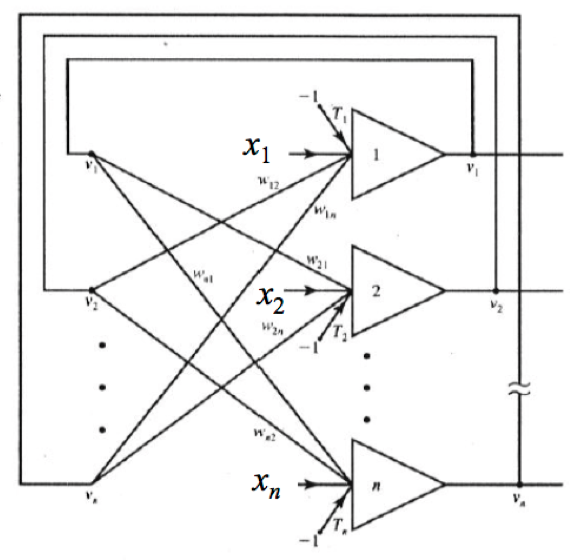
\includegraphics{chapter6_1}
\end{figure}
The total synaptic input:
\begin{equation}
\begin{split}
u_i &= \sum_{j=1,j\ne i}^{n} w_{ij} v_j + x_i -t_i \\
&= \mathbf{w^{T} v} + x_i - t_i
\end{split}
\label{hopfield_input}
\end{equation}
Rewritten in matrix notations:
$$\mathbf{u = W v + x - t}$$
Where matrix $\mathbf{W}$ is called the connectivity matrix:
$$ \mathbf{W}
\begin{bmatrix}
0 & w_{12} & \cdots & w_{1n} \\
w_{21} & 0 & \cdots & w_{2n} \\
\vdots & \vdots & \ddots & \vdots \\
w_{n1} & w_{n2} & \cdots & 0
\end{bmatrix}
$$
\begin{center}where $w_{ij} = w_{ji}$ and $w_{ii} = 0$ \end{center}
The unipolar Hopfield processing unit:
$$v_{i} =
\begin{cases} 
    0 & u_i \le 0 \\
    1 & u_i > 0
\end{cases}
$$
The bipolar Hopfield processing unit:
$$v_{i} =
\begin{cases} 
    -1 & u_i \le 0 \\
    1 & u_i > 0
\end{cases}
$$

\section{Updating Activation of Neurons}
Activity of each neuron of the Hopfield network is usually updated in an asynchronous manner. \\
The energy of node $i$ is defined as:
\begin{equation*}
\begin{split}
E_i &= -v_i u_i \\
&= - v_i \Big(\sum_{j} w_{ij} v_j + x_i - t_i \Big) \\
E &= -\frac{1}{2} \sum_{i=1}^{n} \sum_{j=1, i\ne j}^{n} w_{ji} v_{i} v_{j} - \sum_{i=1}^{n} x_i v_i + \sum_{i=1}^{n} t_i v_i \\
&= -\frac{1}{2} \mathbf{v^{T} W v - v^{T} x + v^{T}t} \\
\nabla E(\mathbf{v}) &= \frac{\partial E(\mathbf{v})}{\partial \mathbf{v}} \\
&= \mathbf{- Wv - x + t} \\
\Delta^{2} E(\mathbf{v}) &= - W
\end{split}
\end{equation*}

\section{Convergence Analysis}
If there is no change in its state, then:
$$\Delta E_i = 0$$
If there is a change in its state, then
\begin{equation}
\begin{split}
\Delta E_i &= E_i^{new} - E_i^{old} \\
&= - (v_i^{new} - v_i^{old}) u_i \\
&= - \Delta v_i u_i 
\end{split}
\label{change_of_energy}
\end{equation}
If $v_i$ change from 0 to 1, then:
$$\Delta v_i = +1\ and\ u_i > 0$$
Substituting to \ref{change_of_energy} yields $\Delta E_i < 0$ \\ \\
If $v_i$ change from 1 to 0, then:
$$\Delta v_i = -1\ and\ u_i \le 0$$
Substituting to \ref{change_of_energy} yields $\Delta E_i < 0$

\section{Hopfield Model Design}

\subsection{Solution by calculation}
By using \ref{hopfield_input} and unipolar Hopfield processing unit, you will get several inequalities. From these inequalities, select one possible solutions. \\
\textit{Note: One of the problems in designing Hopfield network is false energy wells}

\subsection{Solution by learning}
Let the set of $P$ training patterns be:
$${\mathbf{s}(1), \mathbf{s}(2), \ldots, \mathbf{s}(P)}$$
$$\mathbf{s}(i) = s_1(p), s_2(p), \ldots , s_n(p)$$
Training is done using \emph{Hebbian learning rule}:
$$w_{ij} = \sum_{p=1}^{P} (2s_i(p) - 1)(2s_j(p) - 1)$$
\begin{center}for unipolar patterns \end{center}

$$w_{ij} = \sum_{p=1}^{P} s_i(p) s_j(p)$$
\begin{center}for bipolar patterns \end{center}

\noindent \textit{Note: you still need to use inequalities to find the threshold $t$}